\chapter{THE HYPERBOLIC GEOMETRY}

We have now the hypothesis of the acute angle. Two lines in a plane
perpendicular to a third diverge on either side of their common
perpendicular. The sum of the angles of a triangle is less than two
right angles, and the propositions of the last chapter hold without
restriction.

\section{Parallel Lines}

From any point, $P$, draw a perpendicular, $PC$, to a given line,
$AB$, and let $PD$ be any other line from $P$ meeting $CB$ in $D$.
If $D$ move off indefinitely on $CB$, the line $PD$ will approach a
limiting position $PE$.

\begin{figure}[h]
\centering
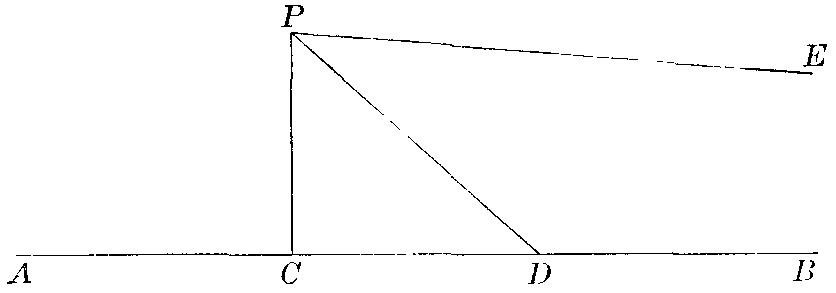
\includegraphics[width=80mm]{fig28.png}
\end{figure}

$PE$ is said to be parallel to $CB$ at $P$. $PE$ makes with $PC$ an
angle, $CPE$, which is called the angle of parallelism for the
perpendicular distance $PC$. It is less than a right angle by an
amount which is the limit of the deficiency of the triangle $PCD$.
On the other side of $PC$ we can find another line parallel to $CA$
and making with $PC$ the same angle of parallelism. We say that $PE$
is parallel to $AB$ towards that part which is on the same side of
$PC$ with $PE$. Thus, at any point there are two parallels to a
line, but only one towards one part of the line. Lines through $P$
which make with $PC$ an angle greater than the angle of parallelism
and less than its supplement do not meet $AB$ at all. We write
$\Pi(p)$ to denote the angle of parallelism for a perpendicular
distance, $p$.

\begin{description}
\item[1.~Theorem.] \emph{A straight line maintains its parallelism
at all points.}

\begin{figure}[h]
\centering
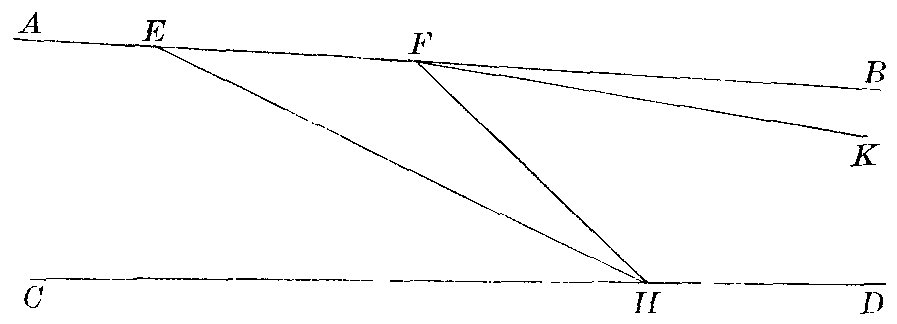
\includegraphics[width=80mm]{fig29.png}
\end{figure}

\textbf{Let} $AB$ be parallel to $CD$ at $E$ and let $F$ be any
other point of $AB$ on either side of $E$, to prove that $AB$ is
parallel to $CD$ at $F$.

\textbf{Proof.} To $H$, on $CD$, draw $EH$ and $FH$. If $H$ move off
indefinitely on $CD$, these two lines will approach positions of
parallelism with $CD$. But the limiting position of $EH$ is the line
$AB$ passing through $F$, and if the limiting position of $FH$ were
some other line, $FK$, $F$ would be the limiting position of $H$,
the intersection of $EH$ and $FH$.

\item[2.~Theorem.] \emph{If one line is parallel to another, the
second is parallel to the first.}

\textbf{Given} $AB$ parallel to $CD$, to prove that $CD$ is parallel
to $AB$.

\textbf{Proof.} Draw $AC$ perpendicular to $CD$. The angle $CAB$
will be acute; therefore, the perpendicular $CE$ from $C$ to $AB$
must fall on that side of $A$ towards which the line $AB$ is
parallel to $CD$ (Chap.~I, II, 1). The angle $ECD$ is then acute and
less than $CEB$, which is a right angle. That is, we have
\begin{equation*}
CAB < ACD, \quad \text{and} \quad CEB > ECD.
\end{equation*}

If the line $CE$ revolve about the point $C$ to the position of
$CA$, the angle at $E$ will decrease to the angle $A$, and the angle
at $C$ will increase to a right angle. There will be some position,
say $CF$, where these two angles become equal; that is,
\begin{equation*}
CFB = FCD.
\end{equation*}

\begin{figure}[h]
\centering
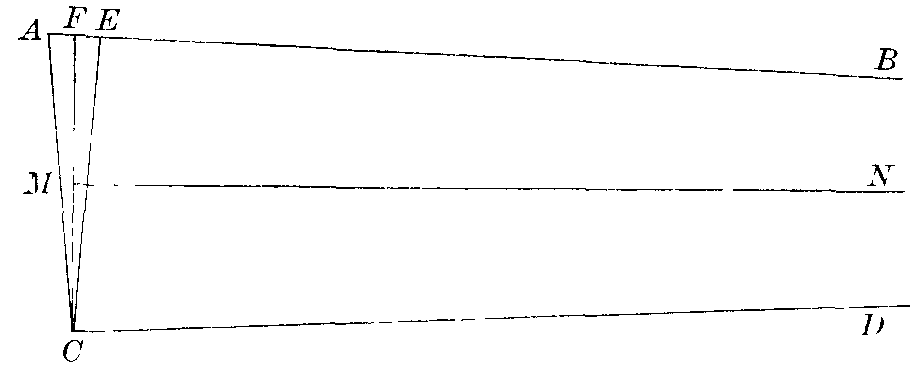
\includegraphics[width=80mm]{fig30.png}
\end{figure}

Draw $MN$ perpendicular to $CF$ at its middle point and revolve the
figure about $MN$ as an axis. $CD$ will fall upon the original
position of $AB$, and $AB$ will fall upon the original position of
$CD$. Therefore, $CD$ is parallel to $AB$.

\textbf{Corollary.} \emph{$FB$ and $CD$ are both parallel to $MN$.}

\begin{figure}[h]
\centering
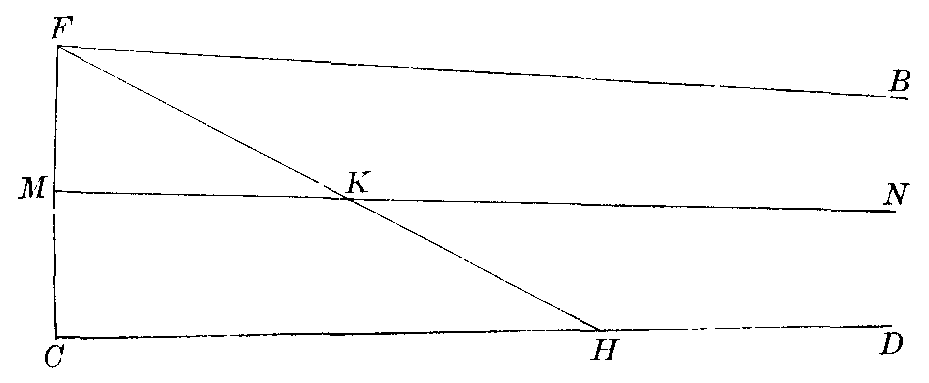
\includegraphics[width=80mm]{fig31.png}
\end{figure}

\textbf{Proof.} $FB$ and $CD$ are symmetrically situated with
respect to $MN$, and cannot intersect $MN$ since they do not
intersect each other. Draw $FH$ to $H$, on $CD$, intersecting $MN$
in $K$. If $H$ move off indefinitely on $CD$, $FH$ will approach the
position of $FB$ as a limit. Now $K$ cannot move off indefinitely
before $H$ does, for $FK < FH$. But again, when $H$ moves off
indefinitely, $K$ cannot approach some limiting position at a finite
distance on $MN$; for $FB$, and therefore $CD$, would then intersect
$MN$ and each other at this point. Therefore, $H$ and $K$ must move
off together, and the limiting position of $FH$ must be at the same
time parallel to $CD$ and $MN$.

In the same way we can prove that any line lying in a plane between
two parallels must intersect one of them or be parallel to both.

\item[3.~Theorem.] \emph{Two lines parallel to a third towards the
same part of the third are parallel to each other.}

\begin{figure}[h]
\centering
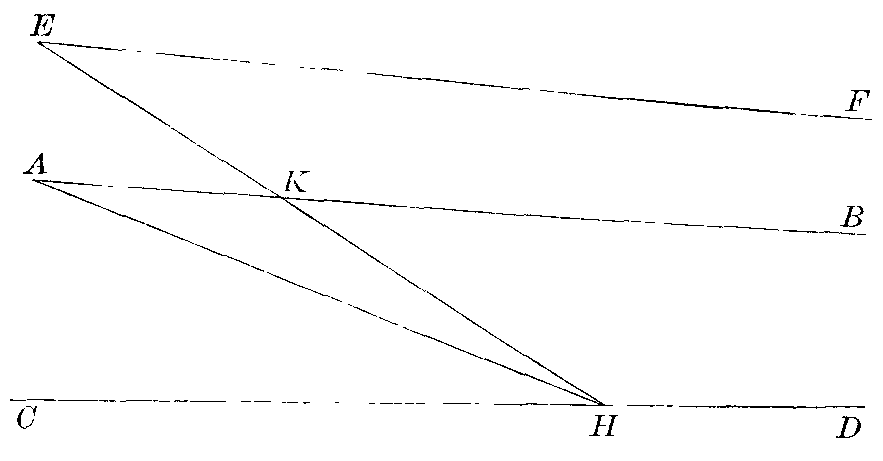
\includegraphics[width=80mm]{fig32.png}
\end{figure}

\textbf{First,} when they are all in the same plane.

\textbf{Let} $AB$ and $EF$ be parallel to $CD$, to prove that they
are parallel to each other.

\textbf{Proof.} Suppose $AB$ lies between the other two. To $H$, any
point on $CD$, draw $AH$ and $EH$, and let $K$ be the point where
$EH$ intersects $AB$. As $H$ moves off indefinitely on $CD$, $AH$
and $EH$ approach as limiting positions $AB$ and $EF$. Now $K$
cannot move off indefinitely before $H$ does, for $EK < EH$. But
again, when H moves off indefinitely, $K$ cannot approach some
limiting position at a finite distance on $AB$; for this point would
be the intersection of $AB$ and $EF$, and the limiting position of
$H$, whereas $H$ moves off indefinitely on $CD$. Therefore, $H$ and
$K$ must move off together, and the limiting position of $EH$ must
be at the same time parallel to $CD$ and $AB$.

If $AB$, lying between the other two, is given parallel to $CD$ and
$EF$, $EF$ must be parallel to $CD$; for a line through $E$ parallel
to $CD$ would be parallel to $AB$, and only one line can be drawn
through $E$ parallel to $AB$ towards the same part.

\begin{figure}[h]
\centering
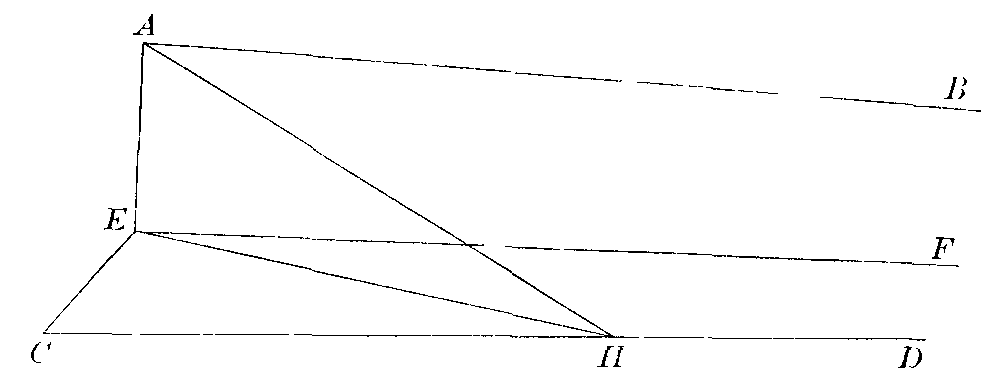
\includegraphics[width=80mm]{fig33.png}
\end{figure}

\textbf{Second}, when the lines are not all in the same plane.

\textbf{Let} $AB$ and $CD$ be two parallel lines and let $E$ be any
point not in their plane.

\textbf{Proof.} To $H$ on $CD$ draw, $AH$ and $EH$. As $H$ moves off
indefinitely, $AH$ approaches the position of $AB$, and the plane
$EAH$ the position of the plane $EAB$. Therefore, the limiting
position of $EH$ is the intersection of the planes $ECD$ and $EAB$.
The intersection of these planes is, then, parallel to $CD$, and in
the same way we prove that it is parallel to $AB$.

Now, if $EF$ is given as parallel to one of these two lines towards
the part towards which they are parallel, it must be the
intersection of the two planes determined by them and the point $E$,
and therefore parallel to the other line also.

\newpage
\item[4.~Theorem.] \emph{Parallel lines continually approach each
other.}

\textbf{Let} $AB$ and $CD$ be parallel, and from $A$ and $B$, any
points on $AB$, drop perpendiculars $AC$ and $BD$ to $CD$. Supposing
that $B$ lies beyond $A$ in the direction of parallelism, we are to
prove that $BD < AC$.

\textbf{Proof.} At $H$, the middle point of $CD$, erect a
perpendicular meeting $AB$ in $K$. The angle $BKH$ is an acute
angle, and the angle $AKH$ is an obtuse angle. Therefore, a
perpendicular to $HK$ at $K$ must meet $CA$ in some point, $E$,
between $C$ and $A$ and $DB$ produced in some point, $F$, beyond
$B$. But $DF = CE$ (Chap.~I, I, 12); therefore, $DB < CA$.

\begin{figure}[h]
\centering
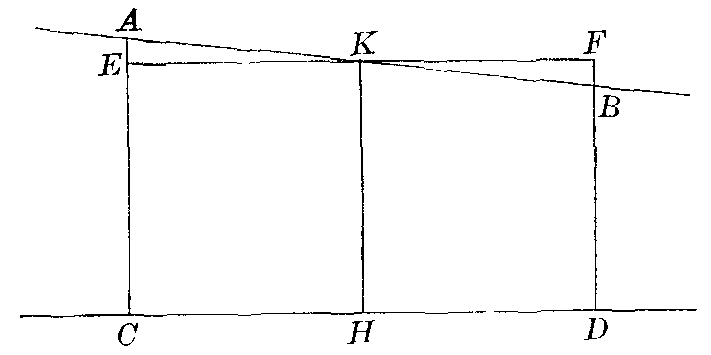
\includegraphics[width=80mm]{fig34.png}
\end{figure}

\textbf{Corollary.} \emph{If $AB$ and $CD$ are parallel and $AC$
makes equal angles with them (like $FC$ in 2 above), then $EF$,
cutting off equal distances on these two lines, $AE = CF$, on the
side towards which, they are parallel, will be shorter than $AC$.}

\begin{figure}[h]
\centering
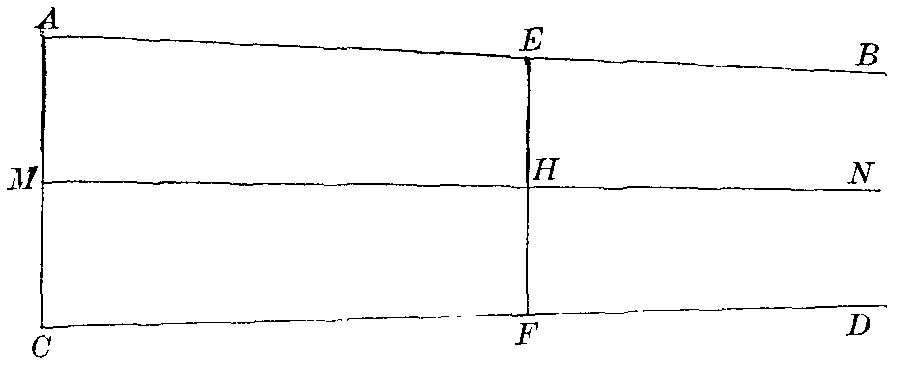
\includegraphics[width=80mm]{fig35.png}
\end{figure}

\textbf{Proof.} $MN$, perpendicular to $AC$ at its middle point, is
parallel to $AB$ and bisects $EF$, the figure being symmetrical with
respect to $MN$. $EH$, the half of $EF$, is less than $AM$, and
therefore $EF$ is less than $AC$.

\item[5.~Theorem.] \emph{As the perpendicular distance varies,
starting from zero and increasing indefinitely, the angle of
parallelism decreases from a right angle to zero.}

\textbf{Proof.} In the first place the angle of parallelism, which
is acute as long as the perpendicular distance is positive, will be
made to differ from a right angle by less than any assigned value if
we take a perpendicular distance sufficiently small.

\begin{figure}[ht]
\centering
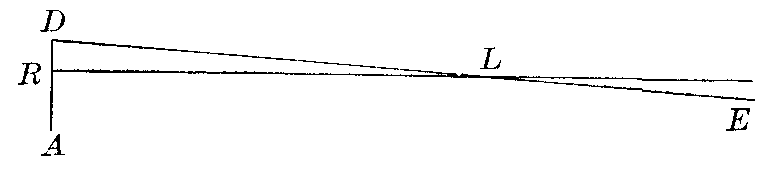
\includegraphics[width=70mm]{fig36.png}
\end{figure}

For, $ADE$ being any given angle as near a right angle as we please,
we can take a point, $L$, on $DE$ and draw $LR$ perpendicular to
$DA$ at $R$. The angle $RDL$ must increase to become the angle of
parallelism for the perpendicular distance $RD$.

\begin{figure}[h]
\centering
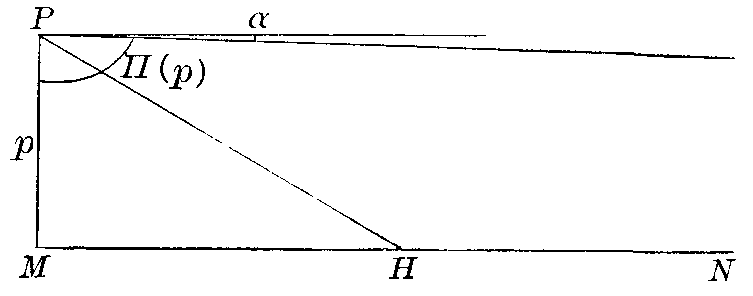
\includegraphics[width=70mm]{fig37.png}
\end{figure}

Now let $p$ be the length of a given perpendicular $PM$, and let
$\alpha$ be the amount by which its angle of parallelism differs
from $\nicefrac{\pi}{2}$; that is, say
\begin{equation*}
\Pi(p) = \frac{\pi}{2} - \alpha.
\end{equation*}
$PM$, being perpendicular to $MN$, and $H$ any point on $MN$, the
angle $MPH$ approaches as a limit the angle of parallelism,
$\Pi(p)$, when $H$ moves off indefinitely on $MN$. The line $PH$
meets the line $MN$ as long as $MPH < \Pi(p)$, and by taking $MPH$
sufficiently near $\Pi(p)$, but less, we can make the angle $MHP$ as
small as we please (see p.~\pageref{p27xref}).

In figure on page~\pageref{p38fig}, let $AC$ be perpendicular to
$AB$, $D$ being any point on $AC$ and $DE$ parallel to $AB$. Draw
$DK$ beyond $DE$, making with $DE$ an angle, $EDK=\Pi(p)$, and make
$DK = p$. $TF$, perpendicular to $DK$ at $K$, will be parallel to
$DE$ and $AB$.

By placing $PM$ of the last figure upon $DKT$, we see that $DC$ will
meet $KT$ in a point, $G$ if
\begin{gather*}
KDC < \Pi(p), \\
\intertext{that is, if}
ADE > 2\alpha.
\end{gather*}

\P~Then in the right triangle $DKG$,
\begin{gather*}
DGK + KDG < \frac{\pi}{2}. \\
\intertext{But}
ADE + KDG = \frac{\pi}{2} + \alpha; \\
\intertext{therefore,}
DGK < ADG - \alpha.
\end{gather*}

\label{p38fig}\begin{figure}[h]
\centering
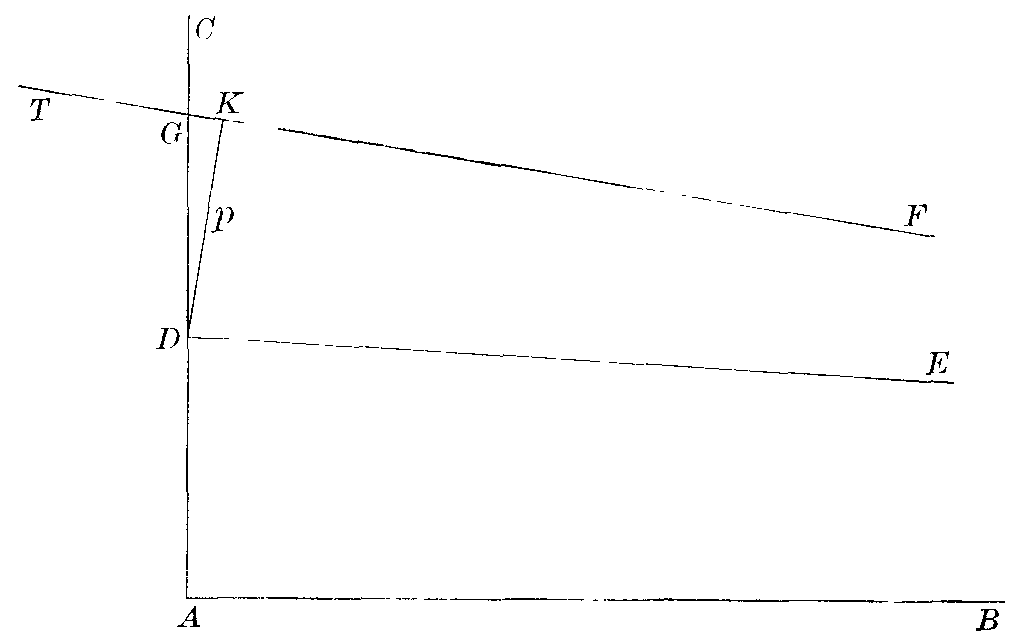
\includegraphics[width=80mm]{fig38.png}
\end{figure}

Starting from the point $G$, we can repeat this construction, and
each time we subtract from the angle of parallelism an amount
greater than $\alpha$. We can continue this process until the angle
of parallelism becomes equal to or less than $2\alpha$.

If the point $D$ move along $AC$, $DE$ remaining constantly parallel
to $AB$, the angle at $D$ will constantly diminish, and by letting
$D$ move sufficiently far on $AC$ we can reach a point where this
angle becomes equal to or less than $2\alpha$.

Suppose $D$ is at the point where the angle of parallelism is just
$2\alpha$. Then, if we draw $DK$ and $TF$ as before, $KT$ will be
parallel to $DC$. All the parallels to $AB$ lying between $AB$ and
this position of $TF$ meet $AC$, and as the parallel moves towards
this position of $TF$, the angle of parallelism at $D$ approaches
zero, and the point $D$ moves off indefinitely.

\begin{figure}[h]
\centering
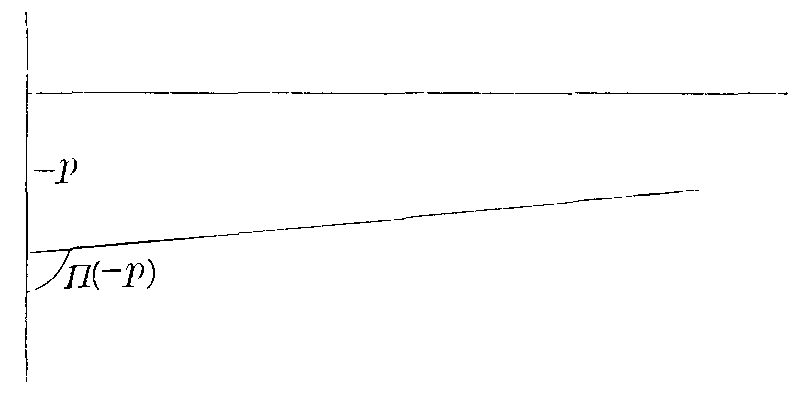
\includegraphics[width=60mm]{fig39.png}
\end{figure}

For an obtuse angle we may take $p$ negative, and we have
\begin{equation*}
\Pi(-p) = \pi - \Pi(p).
\end{equation*}

\item[6.~Theorem.] \emph{The perpendiculars erected at the middle
points of the sides of a triangle are all parallel if two of them
are parallel.}

\begin{figure}[h]
\centering
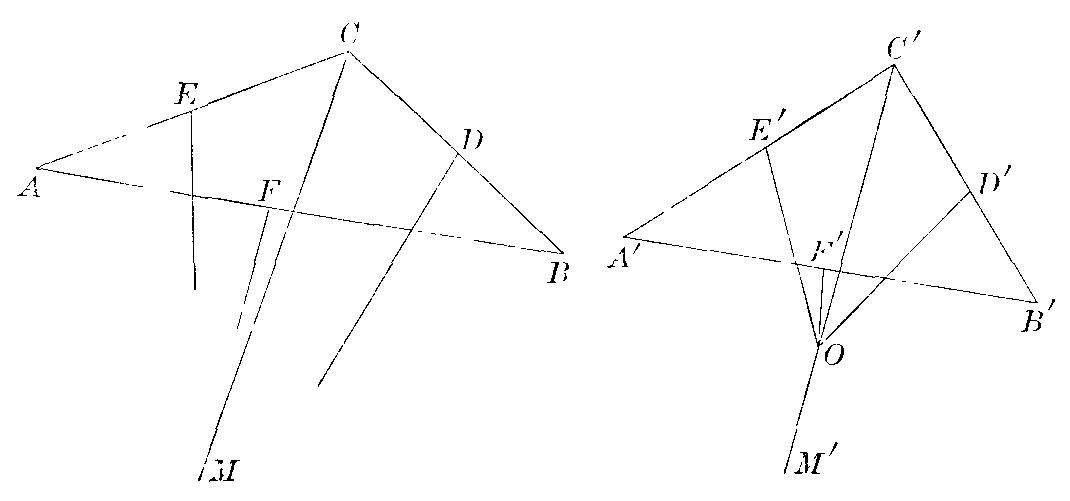
\includegraphics[width=90mm]{fig40.png}
\end{figure}

\textbf{Let} $A$, $B$, and $C$ be the vertices of the triangle, and
$D$, $E$, and $F$, respectively, the middle points of the opposite
sides. Suppose the perpendiculars at $D$ and $E$ are given parallel,
to prove that the perpendicular at $F$ is parallel to them.

\textbf{Proof.} Draw $CM$ through $C$ parallel to the two given
parallel perpendiculars. $CM$ forms with the two sides at $C$ angles
of parallelism $\Pi\left(\dfrac{a}{2}\right)$ and
$\Pi\left(\dfrac{b}{2}\right)$, of which the angle at $C$ is the sum
or difference according as $C$ lies between the given perpendiculars
or on the same side of both. By properly diminishing these angles at
$C$, keeping the lengths of $CA$ and $CB$ unchanged, we can make the
perpendiculars at their middle points $D$ and $E$ intersect $CM$,
and therefore each other, at any distance from $C$ greater than
$\nicefrac{a}{2}$ and greater than $\nicefrac{b}{2}$.

Let $A'B'C'$ be the triangle so formed, $O$ the point where the two
given perpendiculars meet, and $C'M'$ the line through $O$. In the
triangle $A'B'C'$, the three perpendiculars meet at the point $O$
(Chap.~I, I, 5), Now we can let $O$ move off on $C'M'$, the
construction remaining the same. That is, we let the lines $C'A'$
and $C'B'$ rotate about $C'$ without changing their lengths, in such
a manner that the three perpendiculars $D'O$, $E'O$, and $F'O$ shall
always pass through $O$. As $O$ moves off indefinitely, the angles
at $C'$ approach $\Pi\left(\dfrac{a}{2}\right)$ and
$\Pi\left(\dfrac{b}{2}\right)$ as limits, and the three
perpendiculars approach positions of parallelism with $C'M'$ and
with each other. But the triangle $A'B'C'$ approaches as a limit a
triangle which is equal to $ABC$, having two sides and the included
angle equal, respectively, to the corresponding parts of the latter.
Therefore, in $ABC$ the three perpendiculars are all parallel.

\item[7.~Theorem.] \emph{Lines which do not intersect and are not
parallel have one and only one common perpendicular.}

\textbf{Proof.} Let $AB$ and $CD$ be the two lines, and from $A$,
any point of $AB$, drop $AC$ perpendicular to $CD$. If $AC$ is not
itself the common perpendicular, one of the angles which it makes
with $AB$ will be acute. Let this angle be on the side towards $AB$,
so that $BAC < \nicefrac{\pi}{2}$. Draw $AE$ parallel to $CD$ on
this same side of $AC$. The angle $EAC$ is less than $BAC$, since
$AB$ is not parallel to $CD$ and does not intersect it. Let $AH$ be
any line drawn in the angle $EAC$, intersecting $CD$ at $H$. If $H$,
starting from the position of $C$, move off indefinitely on the line
$CD$, the angle $BAH$ will decrease from the magnitude of the angle
$BAC$ to the angle $BAE$. The angle $AHC$ will decrease
\emph{indefinitely} from the magnitude of the angle at $C$, which is
a right angle and greater than $BAC$. There will be some position
for which $BAH=AHC$. In this position the line $NM$ through the
middle point of $AH$ perpendicular to one of the two given lines
will be perpendicular to the other, as proved in Chap.~I, I, 10.

\begin{figure}[h]
\centering
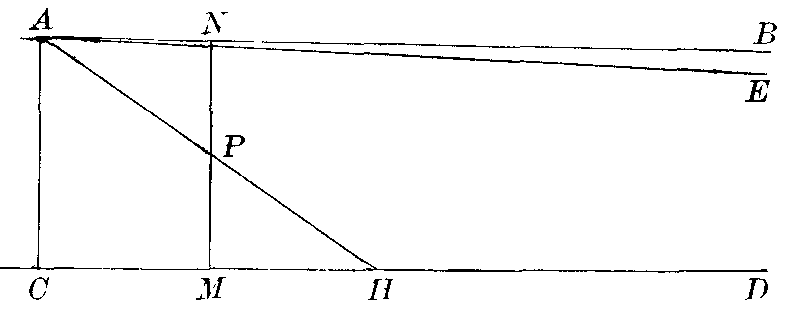
\includegraphics[width=80mm]{fig41.png}
\end{figure}

If there were two common perpendiculars we should have a rectangle,
which is impossible in the Hyperbolic Geometry.

\item[8.~Theorem.] \emph{If the perpendiculars erected at the middle
points of the sides of a triangle do not meet and are not. parallel,
they are all perpendicular to a certain line.}

\begin{figure}[h]
\centering
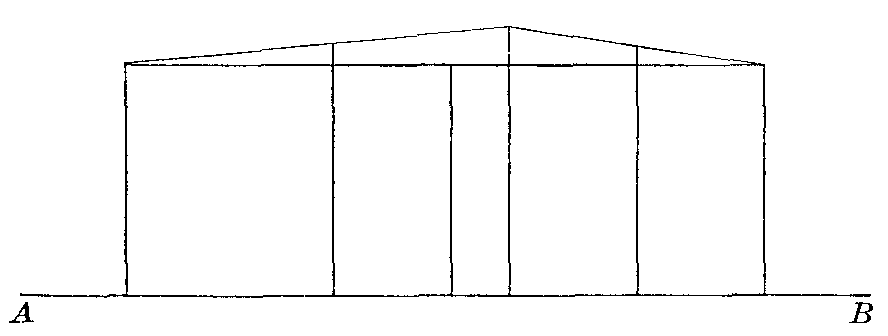
\includegraphics[width=90mm]{fig42.png}
\end{figure}

\textbf{Proof.} We can draw a line, $AB$, that will be perpendicular
to two of these lines, and the perpendiculars from the three
vertices of the triangle upon this line will be equal, by Chap.~I,
II, 13. A perpendicular to $AB$ erected midway between any two of
these three is perpendicular to the corresponding side of the
triangle at its middle point (Chap.~I, I, 11). Thus, all three of
the perpendiculars erected at the middle points of the sides of the
triangle are perpendicular to $AB$.

A line is parallel to a plane if it is parallel to its projection on
the plane.

\item[9.~Theorem.] \emph{A line may be drawn perpendicular to a
plane and parallel to any line not in the plane.}

\begin{figure}[h]
\centering
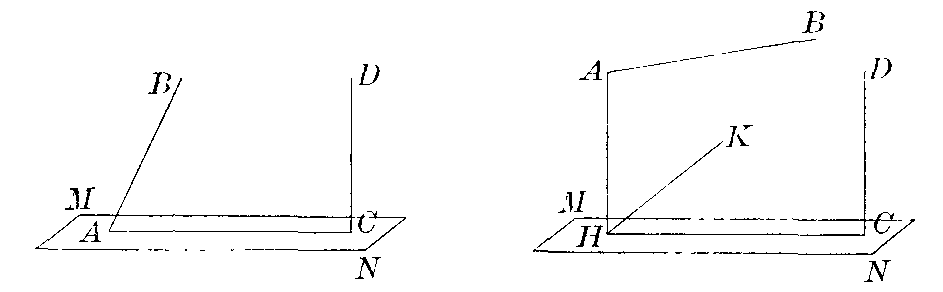
\includegraphics[width=100mm]{fig43.png}
\end{figure}

\textbf{Proof.} Let $AB$ be the given line and $MN$ the plane, if
$AB$ meets the plane $MN$ at a point, $A$, we take on its projection
a length, $AC$, such that the angle at $A$ equals $\Pi(AC)$. Then
$CD$, perpendicular to the plane at $C$, will be parallel to $AB$.
In the same way, on the other side of the plane a perpendicular can
be drawn parallel to $BA$ produced.

If $AB$ does not meet $MN$, then at least in one direction it
diverges from $MN$. Through $H$, any point of the projection of $AB$
on the plane, we can draw a line, $HK$, parallel to $AB$ towards
that part of $AB$ which diverges from $MN$, and then draw $CD$
parallel to this line and perpendicular to the plane.

Unless $AB$ is parallel to $MN$ it will meet the plane at some
point, or the plane and line will have a common perpendicular, and
the line will diverge from the plane in both directions. In the
latter case there are two perpendiculars that are parallel to the
line, one parallel towards each part of the line.

Two perpendiculars cannot be parallel towards the same part of a
line; for then they would be parallel to each other, and two lines
cannot be perpendicular to a plane and parallel to each other.
\end{description}

\newpage
\section{Boundary-curves and Surfaces, and Equ\-i\-dist\-ant-curves
and Surfaces}

Having given the line $AB$, at its extremity, $A$, we take any
arbitrary angle and produce the side $AC$ so that the perpendicular
erected at its middle point shall be parallel to $AB$. The locus of
the point $C$ is a curve which is called oricycle, or
boundary-curve. $AB$ is its axis.

\begin{figure}[h]
\centering
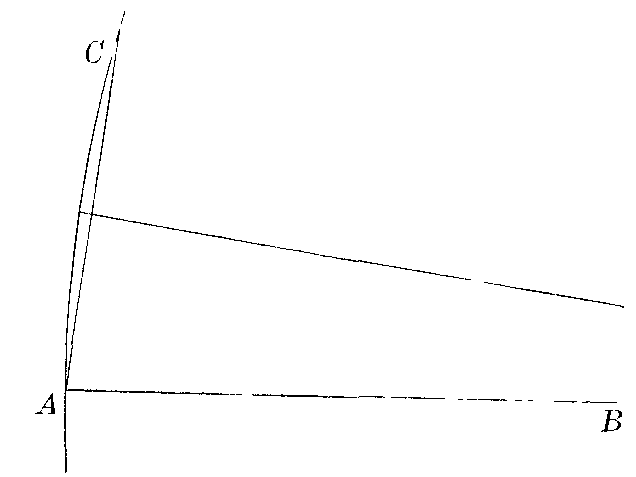
\includegraphics[width=60mm]{fig44.png}
\end{figure}

From their definition it follows that all boundary-curves are equal,
and the boundary-curve is symmetrical with respect to its axis; if
revolved through two right angles about its axis, it will coincide
with itself.

\begin{description}
\item[1.~Theorem.] \emph{Any line parallel to the axis of a
boundary-curve may be taken for axis.}

\textbf{Let} $AB$ be the axis and $CD$ any line parallel to $AB$, to
prove that $CD$ may be taken as axis.

\begin{figure}[h]
\centering
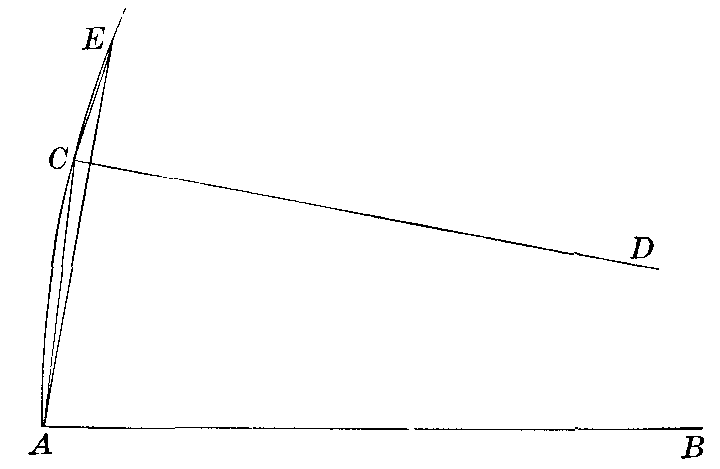
\includegraphics[width=70mm]{fig45.png}
\end{figure}

\textbf{Proof.} Draw $AC$; also to $E$, any other point on the
curve, draw $AE$ and $CE$. The perpendiculars erected at the middle
points of $AC$ and of $AE$ are parallel to $AB$ and $CD$ and to each
other. Therefore, the perpendicular erected at the middle point of
$CE$, the third side of the triangle $ACE$, is parallel to them and
to $CD$. $CD$ then may be taken as axis.

\textbf{Corollary.} \emph{The boundary-curve may be slid along on
itself without altering its shape; that is, it has a constant
curvature.}

\item[2.~Theorem.] \emph{Two boundary-curves having a common set of
axes cut off the same distance on each of the axes, and the ratio of
corresponding arcs depends only on this distance.}

\begin{figure}[h]
\centering
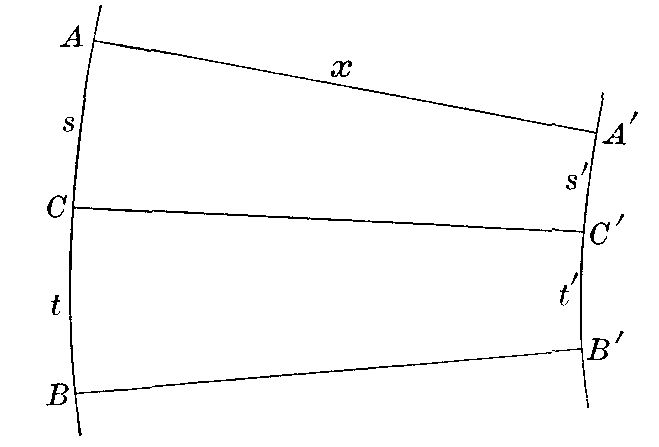
\includegraphics[width=70mm]{fig46.png}
\end{figure}

\textbf{Proof.} Take any two axes and a third axis bisecting the arc
which the first two intercept on one of the two boundary-curves. By
revolving the figure about this axis we show that the curves cut off
equal distances on the two axes.

Let $AA'$, $BB'$, and $CC'$ be any three axes of the two
boundary-curves $AB$ and $A'B'$; let their common length be $x$ and
let them intercept arcs $s$ and $t$ on $AB$, $s'$ and $t'$ on
$A'B'$.

When $s = t$, $s' = t'$, and, in general,
\begin{equation*}
\frac{s}{t} = \frac{s'}{t'},
\end{equation*}
as we prove, first when $s$ and $t$ are commensurable, and then by
the method of limits when they are incommensurable. The ratio
$\nicefrac{s}{s'}$ is, therefore, a constant for the given value of
$x$.

\P~Write $\nicefrac{s}{s'} = f(x).$

\begin{figure}[h]
\centering
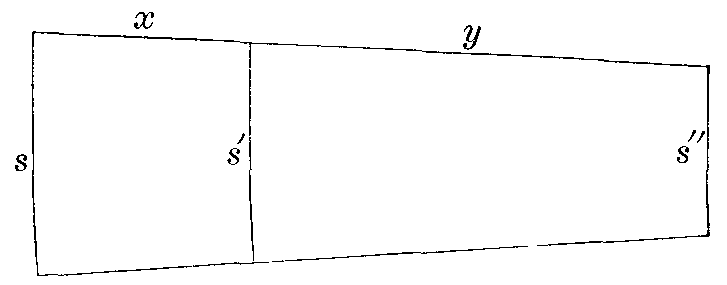
\includegraphics[width=70mm]{fig47.png}
\end{figure}

\label{p45ref}\P~From three boundary-curves having the same set of
axes, we find
\begin{equation*}
f(x+y) = f(x)f(y)
\end{equation*}
This property is characteristic of the exponential function whose
general form is $f(x)= e^{ax}$.\label{p45fn}\footnote{Putting $y =
x$, $2x$, $\cdots$ $(n-1)x$ in succession, we find
\begin{equation*}
f(nx) = [f(x)]^n
\end{equation*}
for positive integer values of $n$, $x$ being any positive quantity.
\par Now
\begin{equation*}
f\left(\frac{r}{s}x\right) = \left[f\left(\frac{x}{s}\right)\right]^r,
\end{equation*}
and this is the $r$th power of the $s$th root of the first member of
the equation
\begin{equation*}
\left[f\left(\frac{x}{s}\right)\right]^s = f(x);\quad \therefore
f\left(\frac{r}{s}x\right) = [f(x)]^\frac{r}{s}.
\end{equation*}
Thus, assuming that $f(x)$ is a continuous function of $x$, we have
proved that for all real positive values of $x$ and $n$
\begin{gather*}
f(nx) = [f(x)]^n, \\
\intertext{and if we put $x$ for $n$ and $1$ for $x$, we have}
f(x) = [f(1)]^x.
\end{gather*}
\par We will write $f(1) = e^a$; then
\begin{equation*}
f(x) = e^{ax}.
\end{equation*}
} Therefore, $\nicefrac{s}{s'}= e^{ax}$, the value of $a$ depending
on the unit of measure (see below p.~\pageref{p76ref}).

\item[3. Theorem.] \emph{The area enclosed by two
boundary-curves having the same axes and by two of their common axes
is proportional to the difference of the intercepted arcs.}

\begin{figure}[h]
\centering
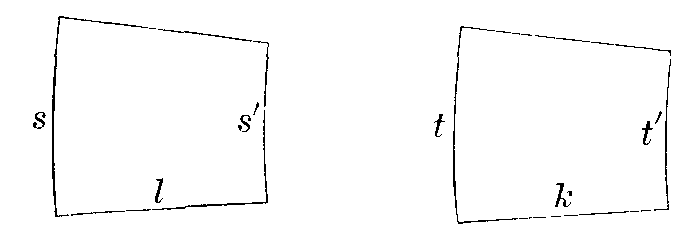
\includegraphics[width=60mm]{fig48.png}
\end{figure}

\textbf{Proof.} Let $s$ and $s'$ be the lengths of the intercepted
arcs, and $l$ the distance measured on an axis between them. Let
$t$, $t'$, and $k$ be the corresponding quantities for a second
figure constructed in the same way.

If the corresponding lines in the two figures are all equal, the
areas are equal, for they can be made to coincide. If only $k = l$,
the areas are to each other as corresponding arcs, say as $s' : t'$,
proved first when the arcs are commensurable, and then by the method
of limits when they are incommensurable.

\newpage
\begin{figure}[h]
\centering
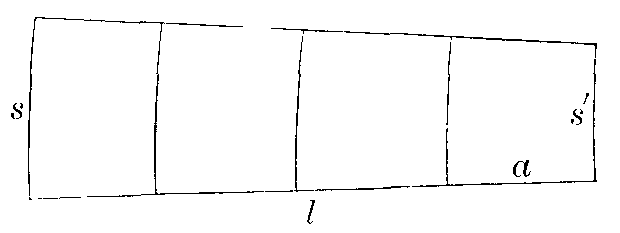
\includegraphics[width=60mm]{fig49.png}
\end{figure}

When $l$ and $k$ are commensurable, suppose
\begin{equation*}
\frac{l}{m} = \frac{k}{n} = a.
\end{equation*}
We can draw a series of boundary-curves at distances equal to $a$ on
the axes and divide the areas into $m$ and $n$ parts, respectively.
If $r$ is the ratio of arcs corresponding to the distance $a$, these
parts will be proportional to the quantities
\begin{gather*}
  s',\ s'r,\ s'r^2,\dots s'r^{m-1};\\
  t',\ t'r,\ t'r^2,\dots t'r^{n-1}.
\end{gather*}

The two areas are then to each other in the ratio
\begin{equation*}
  s' \frac{r^m-1}{r-1} \colon t' \frac{r^n-1}{r-1}.
\end{equation*}

But
\begin{equation*}
  s'r^m = s \text{ and } t'r^n = t,
\end{equation*}
so that this is the same as the ratio
\begin{equation*}
  s-s' \colon t-t'.
\end{equation*}

When $l$ and $k$ are incommensurable, we proceed as in other similar
demonstrations.

This theorem is analogous to the one which we have proved about
polygons: the area is proportional to the amount of rotation in
excess of four right angles in going around the figure, for the rate
of rotation in going along a boundary-curve is constant.

\begin{figure}[h]
\centering
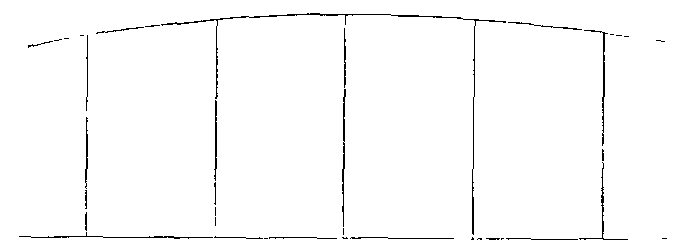
\includegraphics[width=60mm]{fig50.png}
\end{figure}

The locus of points at a given distance from a straight line is a
curve which may be called an equidistant-curve. The perpendiculars
from the different points of this curve upon the base line are equal
and may be called axes of the curve.

An equidistant-curve fits upon itself when revolved through two
right angles about one of its axes or when slid along upon itself.
It has a constant curvature.

It can be proved, exactly as in the case of two boundary-curves
having the same set of axes, that arcs on an equidistant-curve are
proportional to the segments cut off by the axes at their
extremities on the base line or on any other equidistant-curve
having the same set of axes.

\item[4.~Theorem.] \emph{The boundary-curve is a limiting curve
between the circle and the equidistant-curve; it may be regarded as
a circle with infinitely large radius, or as an equidistant-curve
whose base line is infinitely distant.}

\begin{figure}[h]
\centering
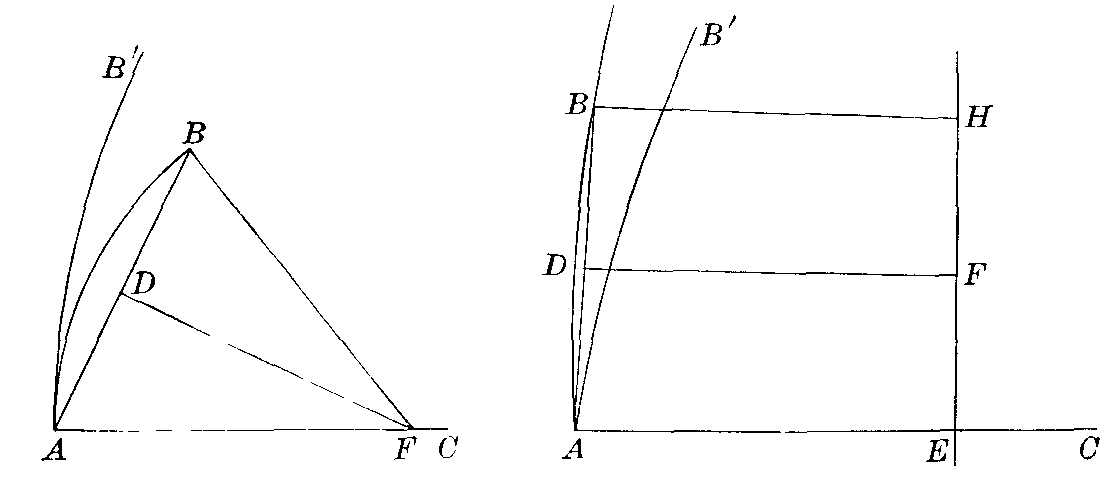
\includegraphics[width=80mm]{fig51.png}
\end{figure}

\textbf{Proof.} Take a line of given length, $AB = 2a$ say, making
an angle, $A$, with a fixed line, $AC$. Construct another angle at
$B$ equal to the angle $A$, and draw a perpendicular to $AB$ at its
middle point, $D$.

If the angle at $A$ is sufficiently small, we have an isosceles
triangle with $AB$ for base, and its vertex at a point, $F$, on
$AC$. With $F$ as centre, we can draw a circle through the points
$A$ and $B$. Now let the angle at $A$ gradually increase, the rest
of the figure varying so as to keep the construction. $F$ will move
off indefinitely, and when $A = \Pi(a)$ the three lines $AF$, $BF$,
and $DF$ will become parallel, and $B$ will become a point on the
boundary-curve $AB'$, which has $AC$ for axis.

On the other hand, if the angle at $A$ were taken acute, but greater
than $\Pi(a)$, we should have three lines, $AE$, $BH$, and $DF$,
perpendicular to a line, $EH$, the base line of an equidistant-curve
through the points $A$ and $B$. Now let the angle $A$ gradually
decrease, the rest of the figure varying so as to preserve the
construction. The quadrilateral $ADFE$, having three right angles
and the fourth angle $A$ decreasing, must increase in area. We get
this same movement if we think of $AD$ and $DF$ remaining fixed in
the plane while $AE$ revolves about $A$, making the angle $A$
decrease. Thus the only way in which the area of the quadrilateral
can increase is for $EH$ to move off along on $AC$ and become more
and more remote from $A$. When $A$ becomes equal to $\Pi (a)$, $BH$
and $DF$ become parallel to $AC$, and $B$ falls on the
boundary-curve $AB'$.
\end{description}

Calling the radius of a circle axis, we find that circles,
boundary-curves, and equidistant-curves have many properties in
common:

The perpendicular erected at the middle point of any chord is an
axis. In particular, a tangent is perpendicular to the axis drawn
from its point of contact. These are curves cutting at right angles
a system of lines through a point, a system of parallel lines, and
the perpendiculars to a given line, respectively.

Two of these curves having the same set of axes cut off equal
lengths on all these axes, and the ratio of corresponding arcs on
two such curves is a constant depending only on the way in which
they divide the axes.

Three points determine one of these curves; that is, through any
three points not in a straight line we can draw a curve which shall
be either a circle, a boundary-curve, or an equidistant-curve, and
through any three points only one such curve can be drawn. Any
triangle may be inscribed in one and only one of these curves.

Each of these curves can be moved on itself or revolved about any
axis through $180^\circ$ into coincidence with itself.

A boundary-surface or orisphere is a surface generated by the
revolution of a boundary-curve about one of its axes.

\begin{description}
\item[5.~Theorem.] \emph{Any line parallel to the axis of a
boundary-surface may be regarded as axis.}

\begin{figure}[h]
\centering
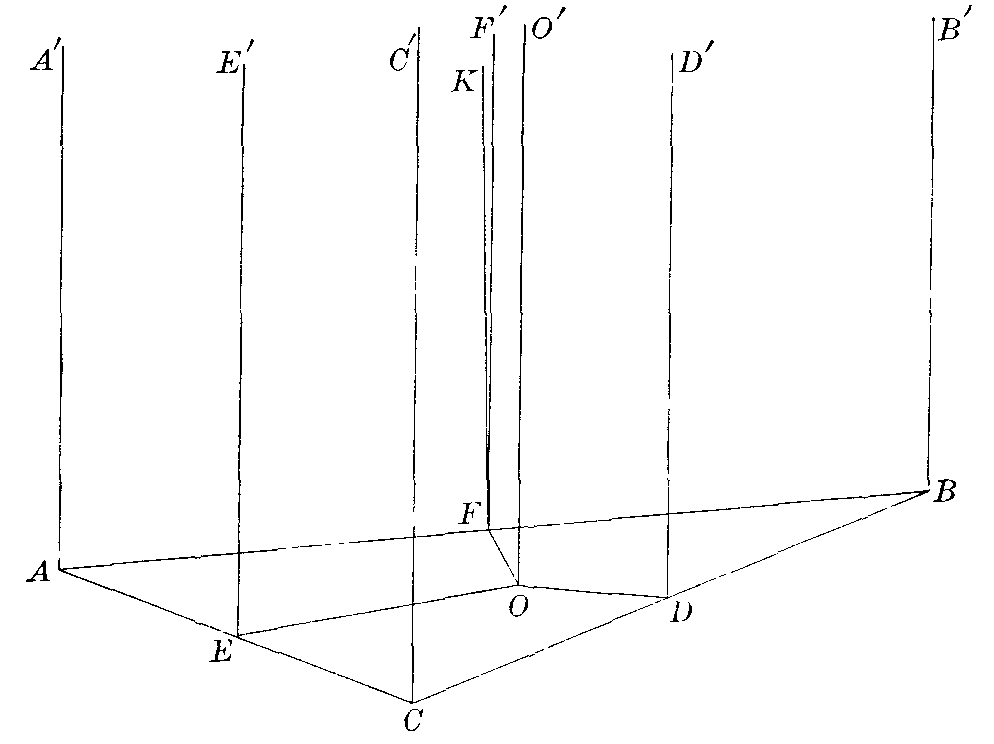
\includegraphics[width=80mm]{fig52.png}
\end{figure}

\textbf{Let} $AA'$ be the axis, meeting the surface at $A$, and
$BB'$ a line parallel to the axis through any other point, $B$, of
the surface; to prove that $BB'$ may be regarded as axis.

\textbf{Proof.} Let $C$ be a third point on the surface. Draw $CC'$
through $C$, and through $D$, $E$, and $F$, the middle points of the
sides of the plane triangle $ABC$, draw $DD'$, $EE'$, and $FF'$ all
parallel to $AA'$. Finally, let $OO'$ be parallel to these lines and
perpendicular to the plane $ABC$. The projecting planes of the other
parallels all pass through $OO'$ (see I, 9).

Since $AA'$ is axis to the surface, $EE'$ and $FF'$ are
perpendicular to $AC$ and $AB$, respectively. Draw $FK$
perpendicular to the plane $ABC$ at $F$. It will lie in the
projecting plane $OFF'$. $AB$, being perpendicular to $FF'$ and to
$FK$, is perpendicular to this plane, $OFF'$, and therefore to $OF$.
In the same way we prove that $AC$ is perpendicular to $OE$.
Therefore, $BC$ is perpendicular to $OD$ (Chap.~I, I, 5). But $OD$
is the intersection of the plane $ABC$ with the plane $ODD'$. Hence,
$BC$ is perpendicular to this plane and to $DD'$ (Chap.~I, II, 15).

$DD'$ being parallel to $BB'$ lies in the plane determined by $BB'$
and $BC$, and in this plane only one perpendicular can be drawn to
$BC$ at its middle point. Therefore, if we pass any plane through
$BB'$ and from $B$ draw a chord to any other point, $C$, of its
intersection with the surface, the perpendicular in this plane to
$BC$, erected at the middle point of $BC$, will be parallel to
$BB'$. This proves that the section is a boundary-curve, having
$BB'$ for axis, and that the surface can be generated by the
revolution of such a boundary-curve around $BB'$.

Therefore, $BB'$ may be regarded as axis of the surface.
\end{description}

A plane passed through an axis of a boundary-surface is called a
principal plane. Every principal plane cuts the surface in a
boundary-curve. Any other plane cuts the surface in a circle; for
the surface may be regarded as a surface of revolution having for
axis of revolution that axis which is perpendicular to the plane.
This perpendicular may be called the axis of the circle, and the
point where it meets the surface, the pole of the circle. The pole
of a circle on a boundary-surface is at the same distance from all
the points of the circle, distance being measured along
boundary-lines on the surface.

Any two boundary-surfaces can be made to coincide, and a
boundary-surface can be moved upon itself, any point to the position
of any other point, and any boundary-curve through the first point
to the position of any boundary-curve through the second point. We
may say that a boundary-surface has a constant curvature, the same
for all these surfaces. Figures on a boundary-surface can be moved
about or put upon any other boundary-surface without altering their
shape or size.

We can develop a Geometry on the boundary-surface. By \emph{line} we
mean the boundary-curve in which the surface is cut by a principal
plane. The angle between two lines is the same as the diedral angle
between the two principal planes which cut out the lines on the
surface.

\begin{description}
\item[6.~Theorem.] \emph{Geometry on the boundary-surface is the
same as the ordinary Euclidean Plane Geometry.}

\textbf{Proof.} On two boundary-surfaces with the same system of
parallel lines for axes corresponding triangles are similar; that
is, corresponding angles are equal, having the same measures as the
diedral angles which cut them out, and corresponding lines are
proportional by (2). But we can place these figures on the same
surface; therefore, on one boundary-surface we can have similar
triangles. Thus, we can diminish the sides of a triangle without
altering their ratios or the angles. We can do this indefinitely;
for the ratio of corresponding lines on the two surfaces, being
expressed by the function $e^{ax}$ of the distance between them, can
be made as large as we please by taking $x$ sufficiently large. If
we assume that figures on the boundary-surface become more and more
like plane figures when we diminish indefinitely their size, it
follows that a triangle on this surface approaches more and more the
form of an infinitesimal plane triangle, for which the sum of the
angles is two right angles, and the angles and sides have the same
relations as in the Euclidean Plane Geometry. All the formulæ of
Plane Trigonometry with which we are familiar hold, then, for
triangles on the boundary-surface.

On the boundary-surface we have the ``hypothesis of the
right angle''. Rectangles can be formed, and the area of a
rectangle is proportional to the product of its base and altitude,
while the area of a triangle is half of the area of a
rectangle having the same base and altitude.
\end{description}

An equidistant-surface is a surface generated by the revolution of
an equ\-i\-dist\-ant-curve about one of its axes. It is the locus of
points at a given perpendicular distance from a plane. Any
perpendicular to the plane may be regarded as an axis, and the
surface is a surface cutting at right angles a system of lines
perpendicular to the plane. The surface has a constant curvature,
fitting upon itself in any position.

\section{Trigonometrical Formulæ}

\begin{description}
\item[1.~Let] $ABC$ be a plane right triangle. Erect $AA'$
perpendicular to its plane and draw $BB'$ and $CC'$ parallel to
$AA'$. Draw a boundary-surface through $A$, having these lines for
axes and forming the boundary-surface triangle $AB''C''$. Also
construct the spherical triangle about the point $B$.

\begin{figure}[h]
\centering
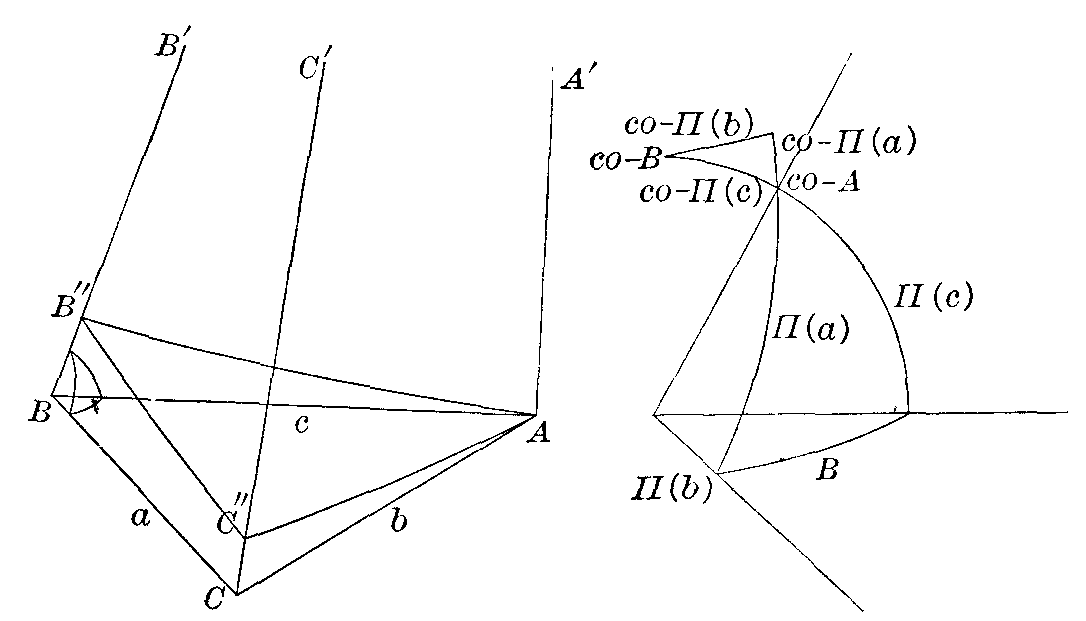
\includegraphics[width=80mm]{fig53.png}
\end{figure}

The angle $A$ is the same in the plane triangle and in the
boundary-surface triangle. The planes through $AA'$ are
perpendicular to $ABC$. Hence, the spherical triangle has a right
angle at the vertex which lies on $c$, and $BC$ being perpendicular
to $CA$ is perpendicular to the plane of $CC'$ and $AA'$. Therefore,
the plane $BCC'$ is perpendicular to the plane $ACC'$, and the
diedral whose edge is $BC$ has for plane angle the angle $ACC'= \Pi
(b)$. Since the boundary-surface triangle is right-angled at $C''$,
the angle $B''$, or what is the same thing, the diedral whose edge
is $BB'$, is the complement of the angle $A$.

In the spherical triangle the side opposite the right angle is $\Pi
(a)$, the two sides about the right angle are $\Pi (c)$ and $B$, and
the opposite angles are $\Pi (b)$ and $90^\circ-A$.

Applying to these quantities the trigonometrical formulæ for
spherical right triangles, we get at once the relations that connect
the sides and angles of plane right triangles.

Produce to quadrants the two sides about the angle whose value is
the complement of $A$. We form in this way a spherical right
triangle in which the side opposite the right angle is the
complement of $\Pi(c)$, the two sides about the right angle are the
complements of $\Pi(a)$ and $\Pi (b)$, and their opposite angles are
the complements of $B$ and $A$. From this triangle we deduce the
following rule for passing from the formulæ of spherical right
triangles to those of plane triangles:

\emph{Interchange the two angles (or the two sides) and everywhere
use the complementary function, tailing the corresponding angle of
parallelism for the sides.}

The formulæ for spherical right triangles are
\begin{gather*}
\begin{aligned}
\sin A &= \frac{\sin a}{\sin c}. & \sin B &= \frac{\sin b}{\sin c}.\\
\cos A &= \frac{\tan b}{\tan c}. & \cos B &= \frac{\tan a}{\tan c}.\\
\tan A &= \frac{\tan a}{\sin b}. & \tan B &= \frac{\tan b}{\sin a}.\\
\sin A &= \frac{\cos B}{\cos b}. & \sin B &= \frac{\cos A}{\cos a}.
\end{aligned}\\
\begin{aligned}
\cos c &= \cos a \cdot \cos b \\
\cos c &= \cot A \cdot \cot B \\
\end{aligned}
\end{gather*}

\newpage
From these, by the rule given on the previous page, we derive the
following formulæ for plane right triangles:
\begin{gather*}
  \begin{aligned}
    \cos B &= \frac{\cos\Pi(a)}{\cos\Pi(c)}. &
    \cos A &= \frac{\cos\Pi(b)}{\cos\Pi(c)}.\\
    \sin B &= \frac{\cot\Pi(b)}{\cot\Pi(c)}. &
    \sin A &= \frac{\cot\Pi(a)}{\cot\Pi(c)}.\\
    \cot B &= \frac{\cot\Pi(a)}{\cos\Pi(b)}. &
    \cot A &= \frac{\cot\Pi(b)}{\cos\Pi(a)}.\\
    \cos B &= \frac{\sin A}{\sin\Pi(b)}. &
    \cos A &= \frac{\sin B}{\sin\Pi(a)}.
  \end{aligned}\\
  \begin{aligned}
    \sin\Pi(c) &= \sin\Pi(a) \sin\Pi(b).\\
    \sin\Pi(c) &= \tan A \tan B.\footnotemark
  \end{aligned}
\end{gather*}
\footnotetext{We can arrange the parts of a right triangle so as to
apply Napier's rules; namely, the arrangement would be

\centering
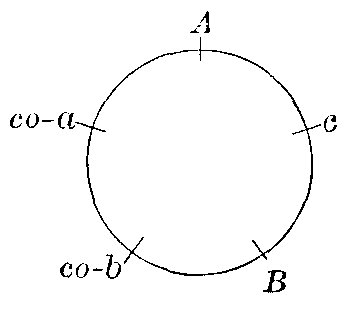
\includegraphics[width=30mm]{fig54.png}}

We can obtain the formulæ for oblique plane triangles by dropping a
perpendicular from one vertex upon the opposite side, thus forming
two right triangles.

\item[2.]~Take the relation
\begin{equation*}
  \sin\Pi(a) = \frac{\sin B}{\cos A}.
\end{equation*}

\textbf{Let} $p$, $q$, and $r$ be the sides of the triangle
$AB''C''$ of our last demonstration and $p'$, $q'$, and $r$ the
corresponding sides of the triangle formed in the same way on a
boundary-surface tangent to the plane $ABC$ at $B$.

\newpage
\begin{figure}[h]
\centering
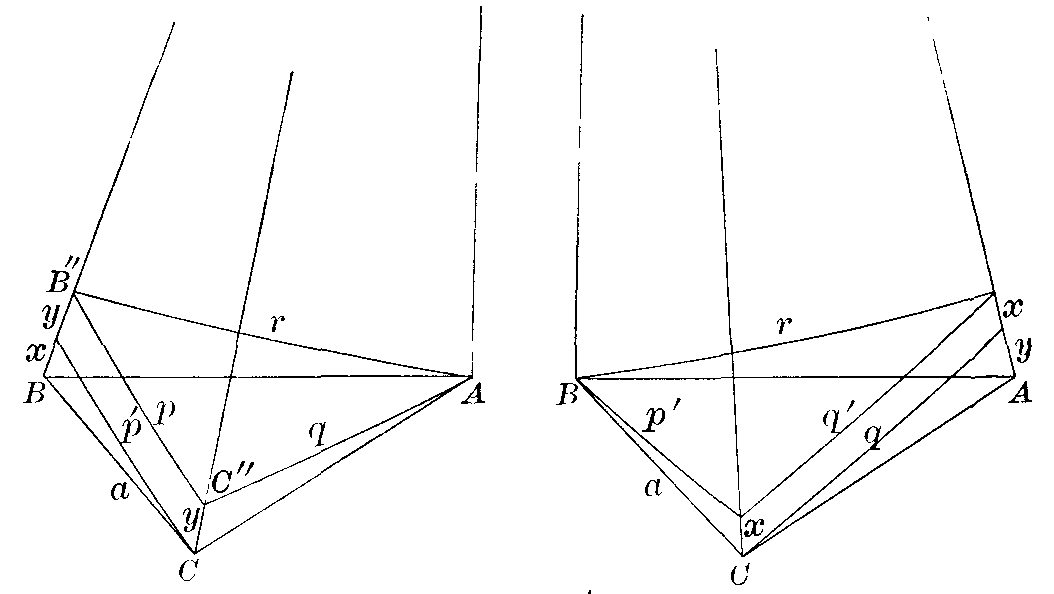
\includegraphics[width=80mm]{fig55.png}
\end{figure}

\begin{align*}
  \sin B &= \frac{q'}{r}, \\
  \cos A &= \frac{q}{r} . \\
  \therefore \sin \Pi(a) &= \frac{q'}{q} .
\end{align*}

\begin{figure}[h]
\centering
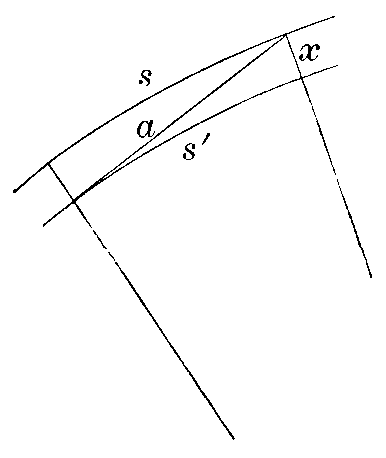
\includegraphics[width=35mm]{fig56.png}
\end{figure}

\label{p56ref}Now $q$ and $q'$ are corresponding arcs on two
boundary-curves which have the same set of parallel lines as axes,
and their distance apart, $x$, is the distance from a boundary-curve
of the extremity of a tangent of arbitrary length, $a$. Thus, we
have for corresponding arcs
\begin{equation*}
  \frac{s'}{s} = \sin \Pi(a)
\end{equation*}

\newpage
\begin{figure}[h]
\centering
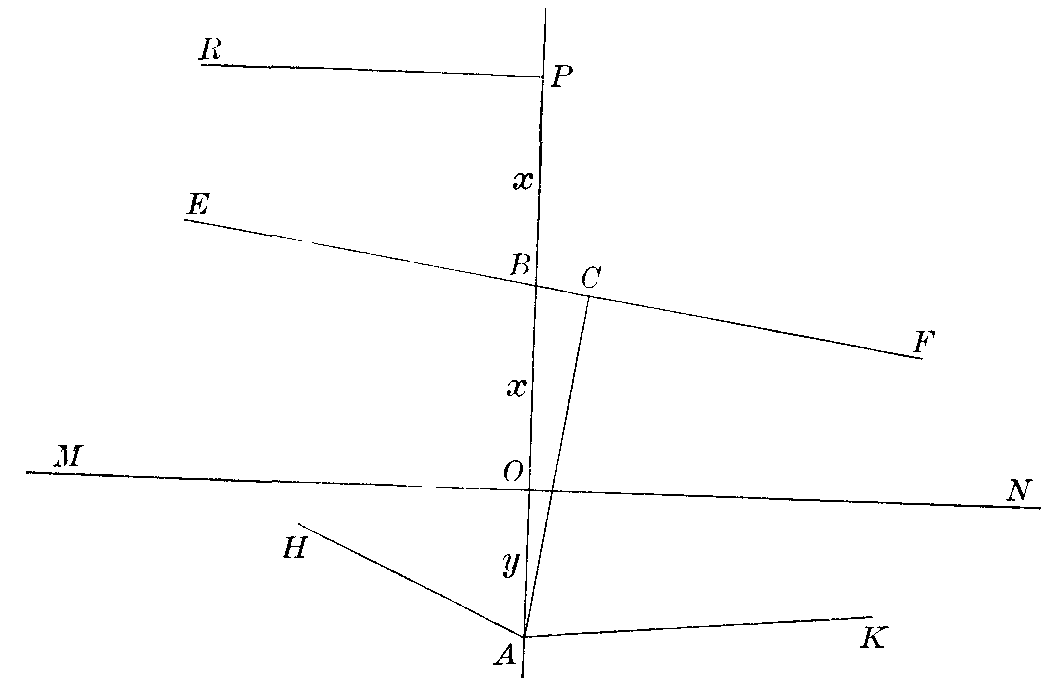
\includegraphics[width=80mm]{fig57.png}
\end{figure}

\item[3.]~To $MN$, a given straight line, erect a perpendicular at a
point, $O$, and on this perpendicular lay off $OA = y$ below $MN$,
and $OB$ and $BP$ each equal to $x$ above $MN$, $x$ and $y$ being
any arbitrary lengths. At $P$ draw $PR$ perpendicular to $OP$ and
extending towards the left, and through $B$ draw $EF$ making with
$OP$ an angle $\Pi (x)$, and therefore parallel on one side to $ON$
and on the other side to $PR$. Finally, draw $AK$ and $AH$, the two
parallels to $EF$ through $A$.

At the point $A$ we have four angles of parallelism:
\begin{align*}
 CAK = CAH &= \Pi (AC),       \\
       OAK &= \Pi (y) ,       \\
       PAH &= \Pi (y+2x) .    \\
\intertext{Therefore, }
   \Pi (y) &= \Pi (AC) + BAC ,\\
\intertext{and}
\Pi (y+2x) &= \Pi (AC) - BAC . \\
\intertext{Now in the right triangle $ABC$}
\cos \Pi (y + x) &= \frac{\cos \Pi (AC)}{\cos BAC} \\
\intertext{or}
  \frac{1-\cos \Pi (y+x)}{1+\cos \Pi (y+x)}
&= \frac{\cos BAC - \cos \Pi (AC)}{\cos BAC + \cos \Pi (AC)}, \\
&= \frac{ \sin \tfrac{1}{2} \left[ \Pi (AC) + BAC \right]
          \sin \tfrac{1}{2} \left[ \Pi (AC) - BAC \right] }
        { \cos \tfrac{1}{2} \left[ \Pi (AC) + BAC \right]
          \cos \tfrac{1}{2} \left[ \Pi (AC) - BAC \right] }; \\
\intertext{whence,}
\tan^2 \tfrac{1}{2} \Pi (y + x)
  &= \tan \tfrac{1}{2} \Pi (y) \tan \tfrac{1}{2} \Pi (y + 2x)
\end{align*}

\P~$\tan \frac{1}{2} \Pi(x)$ is then a function of $x$, say $f(x)$,
satisfying the condition
\begin{align*}
  \left[ f(y + x) \right]^2 & = f(y) f(y+2x) \\
\intertext{or}
  \frac{f(y+x)}{f(y)} & = \frac{f(y+2x)}{f(y+x)}
\end{align*}
and putting successively in this equation $y + x$, $y + 2x$, etc.,
for $y$, we may add
\begin{equation*}
= \frac{f(y+3x)}{f(y+2x)} = \cdots
= \frac{f(y+nx)}{f \left[ y+(n-1)x \right]}
\end{equation*}

\P~$\Pi (0) = \nicefrac{\pi}{2}$ and $\tan \tfrac{1}{2} \Pi (0) =
1$; therefore, putting $y = 0$ in the first and last of all these
fractions, we have
\begin{align*}
  f(x) & = \frac{f(nx)}{f\left[ (n-1) x\right]} , \\
\intertext{or}
  f(nx) & = f\left[(n-1)x \right] f(x). \\
\therefore f(nx) & = \left[ f(x)\right]^n .
\end{align*}

This equation is characteristic of the exponential
function.\footnote{See footnote, p.~\pageref{p45fn}.} $\Pi (x)$
being an acute angle, $tan \tfrac{1}{2} \Pi (x) < 1$; therefore, we
may write $f(1) = e^{-a'}$, so that $f(x) = e^{-a'x}$. $a'$ depends
on the unit of measure; we will take the unit so that $a' = 1$.
Finally, since $\Pi(-x) = \pi - \Pi (x)$,
\begin{equation*}
\tan \tfrac{1}{2} \Pi (-x)
  = \cot \tfrac{1}{2} \Pi (x)
  = \left[ \tan \tfrac{1}{2} \Pi (x) \right]^{-1} .
\end{equation*}
\newpage
That is, for all real values of $x$
\begin{align*}
    \tan \tfrac{1}{2} \Pi (x) &= e^{-x} ,
\intertext{or}
\frac{1-\cos\Pi(x)}{\sin\Pi(x)}
  &= \cos ix + i\sin ix.\footnotemark
\end{align*}\label{p59ref}
\footnotetext{$i$ stands for $\sqrt{-1}$. The best way to get the
relations between the exponential and trigonometrical functions is
by their developments in series:
\begin{align*}
  e^x &= 1 + x + \frac{x^2}{2!} + \dots + \frac{x^n}{n!} + \dotsb,\\
  \cos x &= 1 - \frac{x^2}{2!} + \frac{x^4}{4!} - \dots +
           (-1)^n\frac{x^{2n}}{2n!} + \dotsb,\\
  \sin x &= x - \frac{x^3}{3!} + \frac{x^5}{5!} - \dots +
           (-1)^n\frac{x^{2n+1}}{(2n+1)!} + \dotsb.
\end{align*}
\par These series are convergent for all values of $x$.
\par Putting $ix$ for $x$, we have
\begin{gather*}
  \begin{aligned}
    e^{ix} &= 1 + ix - \frac{x^2}{2!} - \frac{ix^3}{3!} + \dotsb\\
    &= 1 - \frac{x^2}{2!} + \frac{x^4}{4!} - \dots +
    i\left( x - \frac{x^3}{3!} + \frac{x^5}{5!} - \dotsb \right);
  \end{aligned} \\
  \begin{aligned}
\emph{i.e.,}\qquad e^{ix}  &= \cos x + i\sin x.\\
\text{Also}\qquad e^{-ix} &= \cos x - i\sin x.\\
    \therefore \cos x &= \tfrac{1}{2} \left(e^{ix} + e^{-ix}\right),\\
    \sin x &= \tfrac{1}{2i} \left(e^{ix} - e^{-ix}\right).
  \end{aligned}
\end{gather*}
\par Again, putting $ix$ for $x$, we have
\begin{align*}
  e^x &= \cos ix - i\sin ix,\\
  e^{-x} &= \cos ix + i\sin ix;\\
  \intertext{and}
  \cos ix &= \tfrac{1}{2} \left(e^x + e^{-x}\right),\\
  \sin ix &= -\tfrac{1}{2i} \left(e^2 - e^{-x}\right).\\
  \cos ix &= 1 + \frac{x^2}{2!} + \frac{x^4}{4!} + \dotsb,\\
  \sin ix &= ix \left(1 + \frac{x^2}{3!} + \frac{x^4}{5!}
                                                     + \dotsb\right).
\end{align*}
\par For real values of $x$, $\cos ix$ and $\dfrac{\sin ix}{ix}$ are
real and positive, and vary from $1$ to $\infty$ as $x$ varies from
$0$ to $\infty$.
\par In the equation $\cos^2ix + \sin^2ix = 1$, the first term is real
and positive for real values of $x$, the second term is real and
negative; therefore, $\sin ix$ is in absolute value less than $\cos
ix$, and $\tan ix$ is in absolute value less than $1$. $\tan ix$
varies in absolute value from $0$ to $1$ as $x$ varies from $0$ to
$\infty$.}

\P~Changing the sign of $x$, we have
\begin{align*}
\frac{1+\cos\Pi(x)}{\sin\Pi(x)} &= \cos ix - i \sin ix, \\
\intertext{and, adding and subtracting,}
\frac{1}{\sin\Pi(x)} &= \cos ix, \\
\cot\Pi(x) &= -i\sin ix.
\end{align*}

\P~The nature of the angle of parallelism is, therefore, expressed
by the equations
\begin{align*}
\sin\Pi(x) &= \frac{1}{\cos ix}, \\
\tan\Pi(x) &= \frac{i}{\sin ix}, \\
\cos\Pi(x) &= \frac{\tan ix}{i}.
\end{align*}

\item[4.]~Substituting in the formulæ of plane right triangles, we
find that they reduce to those of spherical right triangles with
$ia$, $ib$, and $ic$ for $a$, $b$, and $c$, respectively. The
formulæ of oblique triangles are obtained from those of right
triangles in the same way as on the sphere, and thus all the formulæ
of Plane Trigonometry are obtained from those of Spherical
Trigonometry simply by making this change.

As fundamental formulæ for oblique triangles we write
\begin{gather*}
\frac{\sin A}{\sin ia} = \frac{\sin B}{\sin ib}
                       = \frac{\sin C}{\sin ic}, \\
\cos ia = \cos ib\, \cos ic + \sin ib\, \sin ic\, \cos A, \\
\cos A  = -\cos B\, \cos C + \sin B\, \sin C\, \cos ia.
\end{gather*}

In the notation of the $\Pi$-function, these are
\begin{gather*}
\sin A\, \tan\Pi(a) = \sin B\, \tan\Pi(b) = \sin C\, \tan\Pi(c), \\
\frac{\sin\Pi(b)\,\sin\Pi(c)}{\sin\Pi(a)} =
                             1-\cos\Pi(b)\,\cos\Pi(c)\,\cos A, \\
\cos A = -\cos B\, \cos C + \frac{\sin B\,\sin C}{\sin\Pi(a)}.
\end{gather*}

\item[5.]~Since for very small values of $x$ we have approximately
\begin{gather*}
\sin ix = ix, \\
\cos ix = 1 + \frac{x^2}{2}, \\
\tan ix = ix, \\
\intertext{our formulæ for infinitesimal triangles reduce to}
\frac{\sin A}{a} = \frac{\sin B}{b} = \frac{\sin C}{c}, \\
a^2 = b^2 + c^2 - 2bc\,\cos A, \\
\cos A = -\cos(B+C).
\end{gather*}

\item[6.]~Triangles on an equidistant-surface are similar to their
projections on the base plane; that is, they have the same angles
and their sides are proportional. Thus the formulæ of Plane
Trigonometry hold for any equidistant-surface if with the letters
representing the sides we put, besides $i$, a constant factor
depending on the distance of the surface from the plane.
\end{description}

